%%%%%%%%%%%%%%%%%%%%%%%%%%%%%%%%%%%%%%%%%
% Jacobs Portrait Poster
% LaTeX Template
% Version 1.0 (31/08/2015)
% (Based on Version 1.0 (29/03/13) of the landscape template
%
% Created by:
% Computational Physics and Biophysics Group, Jacobs University
% https://teamwork.jacobs-university.de:8443/confluence/display/CoPandBiG/LaTeX+Poster
% 
% Further modified by:
% Nathaniel Johnston (nathaniel@njohnston.ca)
%
% Portrait version by:
% John Hammersley
%
% The landscape version of this template was downloaded from:
% http://www.LaTeXTemplates.com
%
% License:
% CC BY-NC-SA 3.0 (http://creativecommons.org/licenses/by-nc-sa/3.0/)
%
%%%%%%%%%%%%%%%%%%%%%%%%%%%%%%%%%%%%%%%%%

%----------------------------------------------------------------------------------------
%	PACKAGES AND OTHER DOCUMENT CONFIGURATIONS
%----------------------------------------------------------------------------------------

\documentclass[final]{beamer}

\usepackage[scale=1.24]{beamerposter} % Use the beamerposter package for laying out the poster

\usetheme{confposter} % Use the confposter theme supplied with this template

\setbeamercolor{block title}{fg=black,bg=white} % Colors of the block titles
\setbeamercolor{block body}{fg=black,bg=white} % Colors of the body of blocks
\setbeamercolor{block alerted title}{fg=white,bg=black!50} % Colors of the highlighted block titles
\setbeamercolor{block alerted body}{fg=black,bg=black!10} % Colors of the body of highlighted blocks
% Many more colors are available for use in beamerthemeconfposter.sty

%-----------------------------------------------------------
% Define the column widths and overall poster size
% To set effective sepwid, onecolwid and twocolwid values, first choose how many columns you want and how much separation you want between columns
% In this template, the separation width chosen is 0.024 of the paper width and a 4-column layout
% onecolwid should therefore be (1-(# of columns+1)*sepwid)/# of columns e.g. (1-(4+1)*0.024)/4 = 0.22
% Set twocolwid to be (2*onecolwid)+sepwid = 0.464
% Set threecolwid to be (3*onecolwid)+2*sepwid = 0.708

\newlength{\sepwid}
\newlength{\onecolwid}
\newlength{\twocolwid}
\newlength{\threecolwid}
\setlength{\paperwidth}{36in} % A0 width: 46.8in
\setlength{\paperheight}{48in} % A0 height: 33.1in
\setlength{\sepwid}{0.024\paperwidth} % Separation width (white space) between columns
\setlength{\onecolwid}{0.22\paperwidth} % Width of one column
\setlength{\twocolwid}{0.464\paperwidth} % Width of two columns
\setlength{\threecolwid}{0.708\paperwidth} % Width of three columns
\setlength{\topmargin}{-0.5in} % Reduce the top margin size
%-----------------------------------------------------------

\usepackage{graphicx}  % Required for including images

\usepackage{booktabs} % Top and bottom rules for tables

%----------------------------------------------------------------------------------------
%	TITLE SECTION 
%----------------------------------------------------------------------------------------

\title{Accelerating Artificial Neural Networks on Embedded FPGA with Hybrid Custom Floating-Point and Logarithmic Dot-Product Approximation} % Poster title

\author{Yarib Nevarez} % Author(s)

\institute{Ph.D. candidate at Universit\"at Bremen} % Institution(s)

%----------------------------------------------------------------------------------------

\begin{document}

\addtobeamertemplate{block end}{}{\vspace*{2ex}} % White space under blocks
\addtobeamertemplate{block alerted end}{}{\vspace*{2ex}} % White space under highlighted (alert) blocks

\setlength{\belowcaptionskip}{2ex} % White space under figures
\setlength\belowdisplayshortskip{2ex} % White space under equations

\begin{frame}[t] % The whole poster is enclosed in one beamer frame

\begin{columns}[t] % The whole poster consists of three major columns, the second of which is split into two columns twice - the [t] option aligns each column's content to the top

\begin{column}{\sepwid}\end{column} % Empty spacer column

\begin{column}{\onecolwid} % The first column

%----------------------------------------------------------------------------------------
%	ABSTRACT
%----------------------------------------------------------------------------------------

\begin{alertblock}{ABSTRACT}

We accelerate artificial neural networks (ANN) optimizing the floating-point computation with vector dot-product approximation. The proposed method exploits the intrinsic error resilience of machine learning (ML) algorithms to reduce computational latency, memory footprint, and power dissipation while preserving inference accuracy. To demonstrate our approach, we address a hardware design exploration with convolutional neural networks (CNNs) and spiking neural networks (SNNs).
\end{alertblock}

%----------------------------------------------------------------------------------------
%	INTRODUCTION
%----------------------------------------------------------------------------------------

\begin{block}{Introduction}

%%%%%%% Contributions
We accelerate ANN with a dot-product hardware design based on approximate computing with hybrid custom floating-point and logarithmic number representation. This hardware unit has a quality configurable scheme based on the bit truncation of the synaptic-weight vector. Fig. 1 illustrates the dot-product hardware module with standard floating-point (IEEE 754) arithmetic, and our approach with hybrid custom floating-point as well as logarithmic approximation. As a design parameter, the mantissa bit-width of the weight vector provides a tunable knob to trade-off between efficiency and quality of result (QoR)\cite{han2013approximate}. Since the lower-order bits have smaller significance than the higher-order bits, truncating them may have only a minor impact on QoR \cite{mittal2016survey}. Further on, we can remove completely the mantissa bits in order to use only the exponent of a floating-point representation. Therefore, the most efficient setup and yet the worst-case quality configuration becomes a logarithmic representation, which consequently leads to significant architectural-level optimizations using only adders and shifters for dot-product approximation in hardware. Moreover, since approximations and noise have qualitatively the same effect\cite{venkataramani2015approximate}, we apply noise tolerance plots as an intuitive visual measure to provide insights into the quality degradation of ANN under approximate processing effects.


\end{block}

\end{column} % End of the first column

\begin{column}{\sepwid}\end{column} % Empty spacer column

\begin{column}{\twocolwid} % Begin a column which is two columns wide (column 2)

\begin{columns}[t,totalwidth=\twocolwid] % Split up the two columns wide column

\begin{column}{\onecolwid}\vspace{-.6in} % The first column within column 2 (column 2.1)

%----------------------------------------------------------------------------------------
%	Design
%----------------------------------------------------------------------------------------

\begin{block}{Dot-Product Hardware Block}

\begin{figure}
	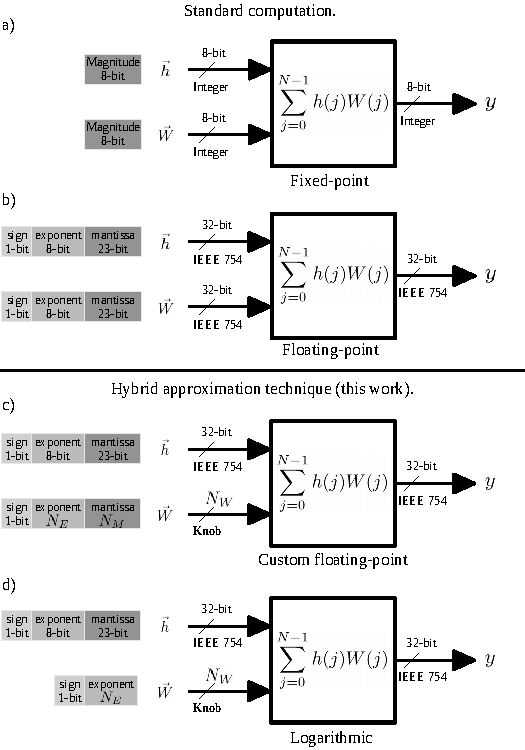
\includegraphics[width=\linewidth]{../figures/dot-product_unit.pdf}
	\caption{Hardware alternatives for vector dot-product.}
	\label{fig:dot_product_unit}
\end{figure}

\end{block}

%----------------------------------------------------------------------------------------

\end{column} % End of column 2.1

\begin{column}{\onecolwid}\vspace{-.6in} % The second column within column 2 (column 2.2)

%----------------------------------------------------------------------------------------
%	SbS
%----------------------------------------------------------------------------------------

\begin{block}{Tensor Processor}
	\begin{figure}
		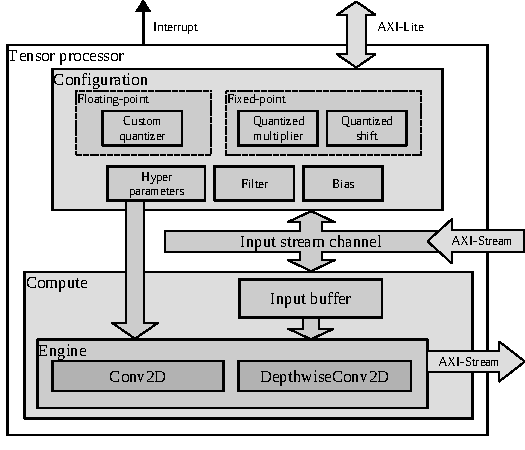
\includegraphics[width=\linewidth]{../figures/accelerator.pdf}
		\caption{Embedded system architecture of the proposed compute platform.}
		\label{fig:conv_sys_design}
	\end{figure}

\end{block}

%----------------------------------------------------------------------------------------

\end{column} % End of column 2.2

\end{columns} % End of the split of column 2 - any content after this will now take up 2 columns width

%----------------------------------------------------------------------------------------
%	IMPORTANT RESULT
%----------------------------------------------------------------------------------------

\begin{alertblock}{Computational intensive operations}
	
\begin{eqnarray} \label{eq:conv2D}
Conv2D\left(W,X\right)_{i,j,o}=\sum_{k,l,m}^{K,L,M}W_{(o,k,l,m)} \cdot X_{(i+k,j+l,m)+b_{o}}
\end{eqnarray}


\begin{eqnarray} \label{eq:dconv2D}
DepthwiseConv2D\left(W,X\right)_{i,j,n}=\sum_{k,l}^{K,L}W_{(k,l,n)} \cdot X_{(i+k,j+l,n)}+b_{n}
\end{eqnarray}

\begin{eqnarray} \label{eq:sbs_update}
h_\mu^{new}(i) = \frac{1}{1+\epsilon} \left(h_\mu(i) + \epsilon \frac{h_\mu(i) W(s_t|i) }{\sum_j h_\mu(j) W(s_t|j)} \right) 
\end{eqnarray}

\end{alertblock} 

%----------------------------------------------------------------------------------------

\begin{columns}[t,totalwidth=\twocolwid] % Split up the two columns wide column again

\begin{column}{\onecolwid} % The first column within column 2 (column 2.1)

%----------------------------------------------------------------------------------------
%	MATHEMATICAL SECTION
%----------------------------------------------------------------------------------------

\begin{block}{Embedded System Platform}
In this section, we present a tensor processor compatible with TensorFlow Lite to accelerate \emph{Conv2D} and \emph{DepthwiseConv2D} operations on embedded FPGA. This implementation is integrated in a hardware/software co-design framework to accelerate tensor operations on FPGAs.

\begin{figure}
	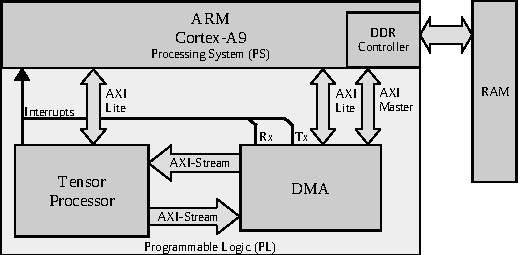
\includegraphics[width=\linewidth]{../figures/system_design.pdf}
	\caption{Embedded system architecture of the proposed compute platform.}
	\label{fig:conv_sys_design}
\end{figure}
\end{block}

%----------------------------------------------------------------------------------------

\end{column} % End of column 2.1

\begin{column}{\onecolwid} % The second column within column 2 (column 2.2)

%----------------------------------------------------------------------------------------
%	RESULTS
%----------------------------------------------------------------------------------------

\begin{block}{Results}

\begin{figure}
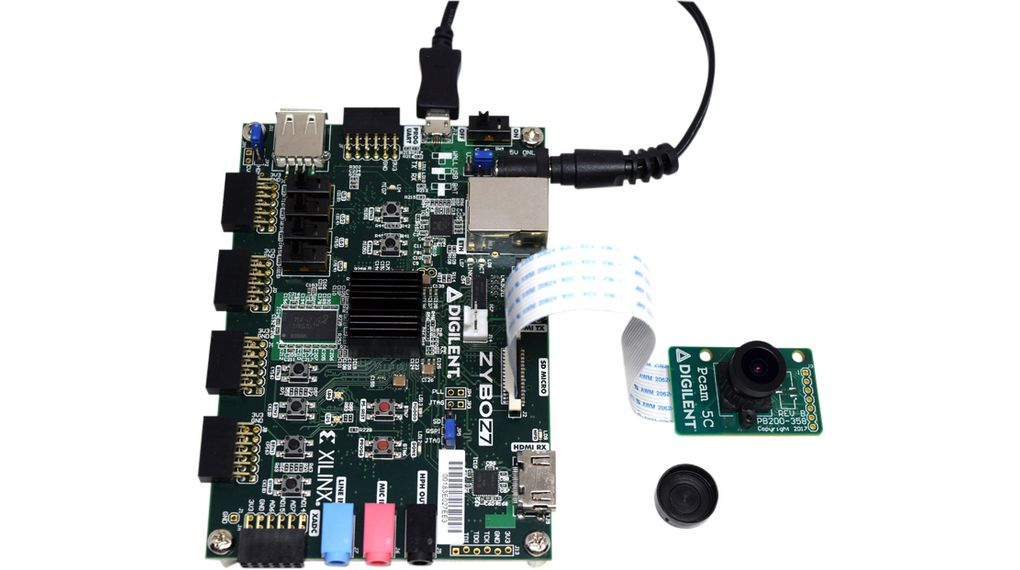
\includegraphics[width=0.8\linewidth]{../figures/placeholder.jpg}
\caption{Figure caption}
\end{figure}

Nunc tempus venenatis facilisis. Curabitur suscipit consequat eros non porttitor. Sed a massa dolor, id ornare enim:

Nunc tempus venenatis facilisis. Curabitur suscipit consequat eros non porttitor. Sed a massa dolor, id ornare enim:

Nunc tempus venenatis facilisis. Curabitur suscipit consequat eros non porttitor. Sed a massa dolor, id ornare enim:

Nunc tempus venenatis facilisis. Curabitur suscipit consequat eros non porttitor. Sed a massa dolor, id ornare enim:

\begin{table}
\vspace{2ex}
\begin{tabular}{l l l}
\toprule
\textbf{Treatments} & \textbf{Res. 1} & \textbf{Res. 2}\\
\midrule
Treatment 1 & 0.0003262 & 0.562 \\
Treatment 2 & 0.0015681 & 0.910 \\
Treatment 3 & 0.0009271 & 0.296 \\
\bottomrule
\end{tabular}
\caption{Table caption}
\end{table}

\end{block}

%----------------------------------------------------------------------------------------

\end{column} % End of column 2.2

\end{columns} % End of the split of column 2

\end{column} % End of the second column

\begin{column}{\sepwid}\end{column} % Empty spacer column

\begin{column}{\onecolwid} % The third column

%----------------------------------------------------------------------------------------
%	CONCLUSION
%----------------------------------------------------------------------------------------

\begin{block}{Spike-by-Spike neural networks}

SbS is a spiking neural network approach based on a
generative probabilistic model. It iteratively finds an estimate of
its input probability distribution $p(s)$ (i.e. the probability of
input node $s$ to stochastically send a spike) by its latent variables
via $r(s) = \sum_i h(i) W(s|i)$. 
where $\vec{h}$ is an inference
population composed of a group of neurons that compete with each
other.



\end{block}

%----------------------------------------------------------------------------------------
%	ADDITIONAL INFORMATION
%----------------------------------------------------------------------------------------

\begin{block}{Additional Information}

Maecenas ultricies feugiat velit non mattis. Fusce tempus arcu id ligula varius dictum. 
\begin{itemize}
\item Curabitur pellentesque dignissim
\item Eu facilisis est tempus quis
\item Duis porta consequat lorem
\end{itemize}

Maecenas ultricies feugiat velit non mattis. Fusce tempus arcu id ligula varius dictum. 
\begin{itemize}
\item Curabitur pellentesque dignissim
\item Eu facilisis est tempus quis
\item Duis porta consequat lorem
\end{itemize}

\end{block}

%----------------------------------------------------------------------------------------
%	REFERENCES
%----------------------------------------------------------------------------------------

\begin{block}{References}

\nocite{*} % Insert publications even if they are not cited in the poster
\small{\bibliographystyle{unsrt}
\bibliography{sample}\vspace{0.75in}}

\end{block}

%----------------------------------------------------------------------------------------
%	ACKNOWLEDGEMENTS
%----------------------------------------------------------------------------------------

\setbeamercolor{block title}{fg=black,bg=white} % Change the block title color

\begin{block}{Acknowledgements}

\small{\rmfamily{Nam mollis tristique neque eu luctus. Suspendisse rutrum congue nisi sed convallis. Aenean id neque dolor. Pellentesque habitant morbi tristique senectus et netus et malesuada fames ac turpis egestas.}} \\

\end{block}

%----------------------------------------------------------------------------------------
%	CONTACT INFORMATION
%----------------------------------------------------------------------------------------

\setbeamercolor{block alerted title}{fg=white,bg=black!50} % Change the alert block title colors
\setbeamercolor{block alerted body}{fg=black,bg=black!10} % Change the alert block body colors

\begin{alertblock}{Contact Information}

\begin{itemize}
\item \href{mailto:nevarez@item.uni-bremen.de}{nevarez@item.uni-bremen.de}
\item \href{www.linkedin.com/in/yarib-nevarez}{linkedin.com/in/yarib-nevarez}
\item \href{https://github.com/YaribNevarez}{github.com/YaribNevarez}
\item +49 (178) 893 6794
\end{itemize}

\end{alertblock}

\begin{center}
\begin{tabular}{ccc}

\includegraphics[width=0.4\linewidth]{../figures/logo_ub_2021.png} & \hfill & 
\includegraphics[width=0.4\linewidth]{../figures/logo_item_ids.png}
\end{tabular}
\end{center}

%----------------------------------------------------------------------------------------

\end{column} % End of the third column

\end{columns} % End of all the columns in the poster

\end{frame} % End of the enclosing frame

\end{document}
